\newpage

\section*{Solutions}

\subsection*{Ex. 1}
This is the required listing
%
\lstset{basicstyle=\scriptsize\sf}
\lstinputlisting{./ex1/sum0.cpp}
\lstset{basicstyle=\sf}
%
Notice that the variable \cpp{temp} is deleted at the end of the \cpp{if} block
inside which it is defined. Similarly the variable \cpp{i} that is used inside
the \cpp{for} loop is not available outside of it. It is common to define the
index of a \cpp{for} loop directly inside the instruction itself like it is done
in the example.

The code can be compiled and executed with the following commands
\begin{verbatim}
g++ -Wall -c sum0.cpp
g++ -o sum0 sum0.o
./sum0
\end{verbatim}
Alternatively the instruction
\begin{verbatim}
g++ -Wall -o sum0 sum0.cpp
\end{verbatim}
compiles the code and performs linking is a single command.
On Unix/Linux systems an executable is not recognized by the extention
\texttt{.exe} like on DOS systems, therefore any extention is suitable, in this
case we chose for an empty one (that is again the common choice).
The parameter \texttt{-Wall} prints to screen almost all the \emph{warnings}.
In this way the compiler reports everything that it finds strange in the code
and that could be the cause of potential errors or problems. It is strongly
adviced to use the flag \texttt{-Wall} every time and read carefully the output.
A good code should not produce any warning at all.

To answer the second point it is sufficient to modify the type of the variable
\cpp{sum} as follows (note that \cpp{0.} is a \emph{floating point} value, while
\cpp{0} is an integer value)
\begin{lstlisting}
int sum = 0;
\end{lstlisting}
The result of the sum of the squares between $1$ and $2000$, stored in
\cpp{sum}, is $-1626300296$. The reason for this misbehavior is due to the fact
that the real value ($2.66867\cdot 10^9$) is above the limit of the storable
values for an integer variable (we triggered an \emph{integer overflow}). In
order to understand why the result is negative, let us consider the case in
which the machine represents an integer with $4$ bytes (e.g.\cpp{sizeof(int)} is
equal to $4$). The biggest positive integer that can be represented is
$2147483647$, with the following binary form
\begin{equation*}
0\quad 1111111~11111111~11111111~11111111
\end{equation*}
where the most significant bit (the leftmost one) is used to set the sign.
Summing $1$ to this value we get
\begin{equation*}
1\quad 0000000~00000000~00000000~00000000
\end{equation*}
that is the representation in two's complement of $-2147483648$, a negative
number. The maximum and minimum value that can be represented for a numeric
type \cpp{T} can be printed to screen using
\begin{lstlisting}
std::cout << std::numeric_limits<T>::max() << " , "
          << std::numeric_limits<T>::min() << std::endl;
\end{lstlisting}
%
\begin{figure}
\centering
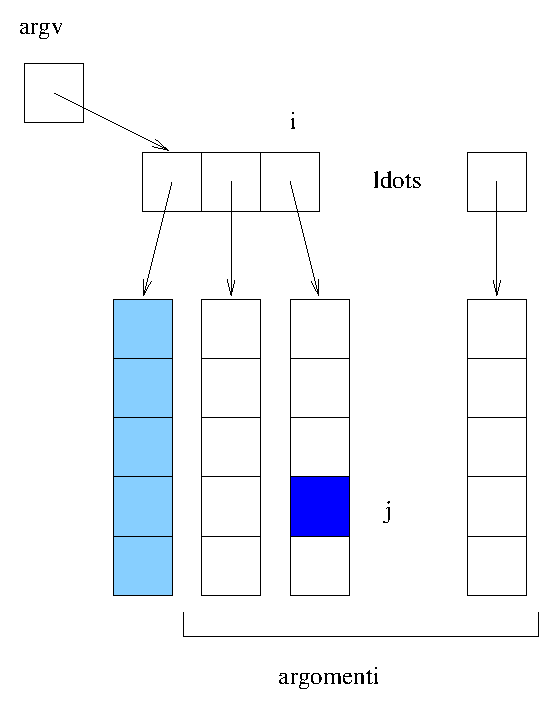
\includegraphics[width=0.4\textwidth]{./figures/tikz/argv}
\caption{\cpp{argv} visual representation. The light blue vector stores the
  name of the executable (in our case it could be \texttt{./sum1}). In blue
  we see the character that corresponds to the call \cpp{argv[i][j]}, where
  \cpp{i} and \cpp{j} are two \cpp{int}.}
\label{fig:argv}
\end{figure}
To answer the third point we use the standard argument for the \cpp{main}
function, \cpp{argc} and \cpp{argv}. The first, \cpp{argc}, is  avariable of
type \cpp{int} that detains the number of arguments that were passed to the
command line. The second, \cpp{argv}, is a vector of c-style character strings,
see \figref{fig:argv}. The first \cpp{argv} element (index $0$) always contains
the executable name, so the parameters are stored starting from index $1$.
Since we are interested in using those parameters as numeric values, we have to
convert the character strings \cpp{argv[1]} and \cpp{argv[2]} to integers. We
can use the function \cpp{atoi} to do it.Note: a vector of character string
pointers can also be interpreted as a matrix of characters, see again 
\figref{fig:argv}.
%
\lstset{basicstyle=\scriptsize\sf}
\lstinputlisting{./ex1/sum1.cpp}
\lstset{basicstyle=\sf}
%
Furthermore, note that the command \cpp{using namespace std} is used to avoid
to specify the qualifier \cpp{std::} to access the objects \cpp{cerr},
\cpp{cout} and \cpp{endl}. The command \cpp{using namespace} must be used with
care, when we are sure that there are no name clashes in the included 
\emph{namespaces}.

\subsection*{Ex. 2}
The listing that is required for the first point is as follows
%
\lstset{basicstyle=\scriptsize\sf}
\lstinputlisting{./ex2/sum1.cpp}
\lstset{basicstyle=\sf}

Note that when we use indices the element numbering in a vector  starts
from $0$ in C++ (as in C). The command \cpp{std::flush} empties the
\emph{output stream buffer}, so the output is phisically performed.
\cpp{std::endl} inserts a \emph{new line} (\cpp{'\n'}) together with a
\cpp{std::flush}.

An alternative way to travel the vector is by using an \emph{iterator}.
Iterators will be throughfully analyzed in the following lessons and are an
extension of the concept of pointer that can be useful to manage standard
library containers. The elements of the vector \cpp{psum} can be printed to
screen using the lines
\lstset{basicstyle=\scriptsize\sf}
\lstinputlisting[linerange={39-41}]{./ex2/sum2.cpp}
\lstset{basicstyle=\sf}

To travel the vector from the last to the first element we can use the
\emph{reverse iterator} of the \cpp{std::vector<double>} type
\lstset{basicstyle=\scriptsize\sf}
\lstinputlisting[linerange={23-24,42-49}]{./ex2/sum3.cpp}
\lstset{basicstyle=\sf}

Note that, differently from the above, a new type psumT has been created with
the command \cpp{typedef}. That type is in fact an \emph{alias} that simplifies
the writing and helps avoiding errors. It becomes usefukl also when there is the
need for a changing the type for the partial sums, since it would be sufficient
to redifine properly the derived type \cpp{psumT}.

The modifications that are required for the third point is implemented in the
following lines that replace the same one in the listing for the first point
\lstset{basicstyle=\scriptsize\sf}
\lstinputlisting[linerange={24-31}]{./ex2/sum2.cpp}
\lstset{basicstyle=\sf}

If the elements were inserted with the \cpp{operator[]} instead of using the
\cpp{push\_back} member at the end the length of the vector would have been
zero (\cpp{psum.size() = 0}) and we would not be able to access the partial
sums. This happens because the \cpp{reserve} member only reserves the memory,
but does not allocate it.

The assignement of the first 10 elements of \cpp{psum} can be performed with
the assign member, that takes as input two iterators that are used as the first
and last location from which to copy
\lstset{basicstyle=\scriptsize\sf}
\lstinputlisting[linerange={51-57}]{./ex2/sum3.cpp}
\lstset{basicstyle=\sf}

